\documentclass{standalone}
% 

% \pgfmathdeclarefunction{gauss}{2}{%
%   \pgfmathparse{1/(#2*sqrt(2*pi))*exp(-((x-#1)^2)/(2*#2^2))}%
% }


\usepackage{pgfplots}
\begin{document}
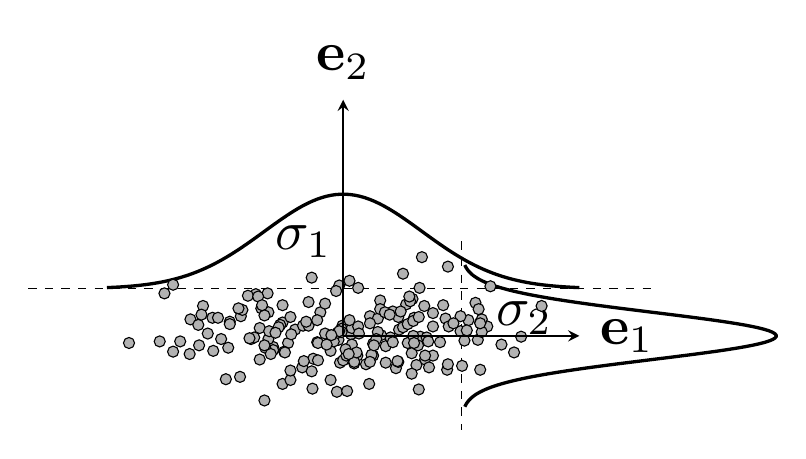
\begin{tikzpicture}[>=stealth]
% define normal distribution function 'normaltwo'
    \def\normaltwo{\x,{4*1/exp(((\x-0)^2)/2)}}
    
    \begin{scope}[rotate = 0]
        \begin{scope}[yscale = .3, yshift = 2cm]
            \draw[color=black,,domain=-3:3, samples = 100, very thick] plot (\normaltwo) node[right] {};
            \draw [dashed] (-4, 0)  --  (4, 0);
            \node [scale = 2] at (-.5, 2) {${\sigma}_1$};
        \end{scope}

        \begin{scope}[yscale = .3, xscale = 1, yshift = 0cm, xshift = 1.5cm, rotate = -90]
            \draw[color=black,,domain=-3:3, samples = 100, very thick] plot (\normaltwo) node[right] {};
            \draw [dashed] (-4, 0)  --  (4, 0);
            \node [scale = 2]  at (-.75, .8) {${\sigma}_2$};
        \end{scope}

     
            \foreach \x/\y in {-1.06/-0.30, 0.54/-0.13, -1.65/-0.19, -0.61/0.08, 0.96/-0.68, 0.83/-0.09, 0.34/0.25, -0.33/-0.08, 1.14/0.29, 0.63/0.31, -0.16/-0.19, 0.10/0.02, 1.74/-0.43, -2.33/-0.07, 0.14/-0.35, 1.74/0.17, -1.17/-0.04, -0.29/0.30, 0.08/0.70, 0.38/-0.25, 0.44/0.22, 1.83/0.12, -1.31/-0.52, 2.01/-0.11, -0.51/0.13, 0.80/0.40, 1.59/0.20, -1.04/0.35, -1.44/0.18, 1.68/0.42, -1.66/0.23, -0.08/-0.71, -0.13/-0.03, -0.89/-0.14, 1.30/0.22, 1.04/-0.30, 1.33/0.88, 0.98/-0.01, -0.44/0.13, -0.95/0.30, -0.01/0.13, -0.06/-0.05, -1.06/0.10, -1.83/-0.12, -0.23/0.41, 1.23/-0.08, 0.87/-0.22, -0.89/-0.18, 0.38/-0.10, -1.94/0.21, 0.13/0.11, 0.18/-0.25, 0.60/-0.02, 0.11/-0.11, 1.49/0.06, 1.49/0.25, -1.44/0.15, 0.82/-0.09, -1.31/0.33, -0.04/-0.34, 0.90/0.23, 2.26/-0.01, 0.48/0.01, 1.06/-0.02, -0.70/-0.09, -0.44/0.43, 1.03/0.38, -1.00/0.26, -0.00/-0.31, 1.71/-0.05, 0.88/0.47, -1.49/-0.55, 0.93/-0.37, 0.87/-0.48, -1.11/0.53, 1.34/0.12, 0.67/-0.41, -0.39/-0.67, 1.76/0.05, -1.95/-0.23, 1.76/0.21, 0.71/0.08, -0.77/-0.61, 0.44/0.05, 0.89/0.00, -0.38/-0.29, -0.80/0.14, 2.17/-0.21, 0.85/0.44, -0.77/0.17, 0.34/0.16, 0.76/0.11, 0.33/-0.61, 0.47/0.45, 0.97/0.61, 2.52/0.38, -1.21/0.51, 1.54/-0.06, -0.66/0.02, 1.57/0.07, 0.95/-0.12, -0.99/-0.15, 0.04/-0.25, -0.92/-0.23, 0.76/0.79, 1.40/0.16, -1.78/0.38, -0.52/-0.40, -1.55/-0.04, -1.46/-0.15, 1.27/0.39, -0.40/-0.45, -0.77/0.39, 0.84/0.50, -1.30/0.25, 1.74/0.16, -0.17/0.00, -0.67/-0.56, 1.32/-0.43, 0.36/-0.24, -1.28/0.33, -1.00/-0.82, 0.47/0.34, 1.14/0.12, 1.14/-0.25, 0.42/-0.04, -1.72/0.03, 0.14/-0.33, -2.16/-0.20, -0.32/-0.31, -0.02/0.09, 0.82/0.15, 1.09/-0.40, 1.08/-0.07, -1.84/0.14, -0.12/-0.07, 1.87/0.63, 1.72/0.34, -0.07/0.04, -2.72/-0.09, -0.96/0.54, -2.07/-0.07, -0.40/0.74, -1.13/-0.02, -0.95/-0.04, -0.80/0.14, -1.08/0.50, 0.53/0.30, 0.70/0.24, 0.39/-0.12, 0.29/-0.36, 0.90/-0.09, -0.75/-0.20, -1.33/0.35, -0.94/0.06, 0.59/0.27, 1.04/-0.25, -0.82/0.11, 0.70/-0.33, 0.73/0.31, 0.63/-0.08, 0.89/0.19, -2.27/0.54, -0.05/0.64, -0.32/-0.09, -1.80/0.27, 0.11/0.10, -0.74/-0.21, -0.67/-0.44, -0.47/0.18, 0.54/-0.34, -0.02/0.05, -1.03/0.39, 0.69/-0.32, 1.51/-0.38, 0.96/0.24, -1.59/0.23, 1.33/-0.36, -0.21/-0.11, -0.86/0.04, -1.19/-0.03, -0.16/-0.56, 0.17/-0.21, -0.67/0.24, -0.50/-0.32, -0.05/0.06, 0.34/-0.33, -0.23/0.03, -2.16/0.65, -0.09/0.57, 0.05/-0.70, -0.33/0.20, -1.00/-0.12, -0.15/0.01, 0.19/0.61, 0.03/-0.17, 0.07/-0.23, 0.19/0.12, 0.08/0.20, 0.20/0.03, }{
            \draw [fill = gray!60] (\x, \y) circle (2pt);
        }

        \draw[->, thick, black] (0,0)  --  (3,0) node[right, scale = 2] {$\mathbf{e}_1$};
        \draw[->, thick, black] (0,0)  --  (0,3) node[above, scale = 2] {$\mathbf{e}_2$};

    \end{scope}

    % \begin{scope}[rotate = 0]
    %     \draw[->, thick] (0,0)  --  (3,0) node[right] {$\mathbf{e}_1$};
    %     \draw[->, thick] (0,0)  --  (0,3) node[above] {$\mathbf{e}_2$};
    %     \begin{scope}[yscale = .6, xscale = .5, yshift = -4cm, yscale = -1]
    %         \draw[color= green!70!black, domain=-3:3, samples = 100, very thick] plot (\normaltwo) node[right] {};
    %         \draw [dashed] (-4, 0)  --  (4, 0);
    %         \node at (0, 2) {$\sigma_1$};
    %     \end{scope}

    %     \begin{scope}[yscale = .85, xscale = .35, yshift = 0cm, xshift = 1cm, rotate = -90]
    %         \draw[color= green!70!black,domain=-3:3, samples = 100, very thick] plot (\normaltwo) node[right] {};
    %         \draw [dashed] (-3, 0)  --  (3, 0);
    %         \node at (.51, 2) {$\sigma_2$};
    %     \end{scope}

     
           
    % \end{scope}
\end{tikzpicture}
\end{document}